\documentclass[a4paper]{amsart}

\usepackage{color}
\usepackage[colorlinks=true, citecolor=red]{hyperref}  %needs to come before amsrefs package to work with \cite{}*{}
\usepackage{amssymb,latexsym}
\usepackage[alphabetic]{amsrefs}
\usepackage[mathscr]{eucal}
\usepackage{pdfsync}
\usepackage{graphicx}
\usepackage{epstopdf}
\DeclareGraphicsRule{.tif}{png}{.png}{`convert #1 `dirname #1`/`basename #1 .tif`.png}
\usepackage[all]{xy}
\usepackage{titletoc}
\usepackage{txfonts}   %  \fint  for integral average

%\usepackage{showkeys}  %options notref  notcite 

%\input{rgb.tex}

%\textcolor{DarkRed}{text in DarkRed}


\CompileMatrices

\theoremstyle{plain}
\newtheorem{theorem}{Theorem}[section]
\newtheorem{lemma}[theorem]{Lemma}
\newtheorem{proposition}[theorem]{Proposition}
\newtheorem{corollary}[theorem]{Corollary}

\theoremstyle{definition}
\newtheorem{definition}[theorem]{Definition}%[section]


\theoremstyle{remark}
\newtheorem{defn}[theorem]{Definition} 
\newtheorem{example}[theorem]{Example}
\newtheorem{remark}[theorem]{Remark}
\newtheorem{discussion}[theorem]{Discussion}

%\numberwithin{equation}{section}

%\newcommand{\abs}[1]{\lvert#1\rvert}

\DeclareMathOperator{\Lip}{Lip}
\DeclareMathOperator{\dist}{dist}
\DeclareMathOperator{\expected}{\mathbb{E}}
\DeclareMathOperator{\prb}{Prob}
\DeclareMathOperator{\spt}{spt}
\DeclareMathOperator{\lap}{\Delta}
\DeclareMathOperator{\Tr}{Tr}
\DeclareMathOperator{\var}{var}
\DeclareMathOperator{\card}{card}

\raggedbottom

%\addtolength{\textwidth}{2cm}
%\addtolength{\oddsidemargin}{-1cm}
%\addtolength{\evensidemargin}{-1cm} 
%\addtolength{\topmargin}{-1cm} 
%\addtolength{\textheight}{2cm}

 
%%% BEGIN DOCUMENT
\begin{document}

\title{Probability Basics}  
\author{John E.\ Hutchinson}
\date{\today}

%\begin{abstract} 
%This is the abstract
%\end{abstract}

\maketitle

\tableofcontents


%%%%%%%%%%%%%%%%%%%%%%%%%%%%%%%%
%%%%%%%%%%%%%%%%%%%%%%%%%%%%%%%%
%%%%%%%%%%%%%%%%%%%%%%%%%%%%%%%%
%%%%%%%%%%%%%%%%%%%%%%%%%%%%%%%%
\section{Set Theoretic material} 

 For a sequence $ (A_n) $ of subsets of a set $ X $ define
 \begin{equation} \label{df} 
 \liminf_{n\to \infty} A_n = \bigcup_{n \geq 1}\bigcap_{m\geq n} A_m,  \quad
 \limsup_{n\to \infty}  A_n = \bigcap_{n \geq 1}\bigcup_{m\geq n} A_m.
\end{equation} 
 Note
\begin{equation} \label{lim} 
 \bigcap_{m\geq n} A_m  \uparrow \liminf_{n\to \infty}  A_n ,  \quad
  \bigcup_{m\geq n} A_m  \downarrow \limsup_{n\to \infty}  A_n,   \quad \text{as } n \to \infty.
\end{equation} 


 In words, 
\begin{equation} \label{words} 
x \in \liminf_{n\to \infty} A_n \Longleftrightarrow  x \in A_n \text{ eventually}, \quad 
x \in \limsup_{n\to \infty} A_n \Longleftrightarrow  x \in A_n \text{ i.o.} 
\end{equation}  
  In particular,   $  \liminf A_n $  is the smallest set detectible by tail events and $  \limsup A_n $  is the largest. 

Clearly,
\begin{equation} \label{dm} 
(\liminf A_n)^c = \limsup  A_n^c, \quad (\limsup A_n)^c = \liminf A_n^c.
\end{equation} 
That is
\begin{equation} \label{}
\neg (A_n \text{ eventually}) \Longleftrightarrow   A_n^c \text{ i.o.}, \quad 
\neg (A_n \text{ i.o.}) \Longleftrightarrow   A_n^c \text{ eventually}.
\end{equation} 

 
\bigskip
  In terms of \emph{indicator} or \emph{characteristic} functions,
\begin{equation} \label{in1} 
\boldsymbol{1}_{\liminf_n A_n } = \liminf_n  \boldsymbol{1}_{A_n}, \quad 
\boldsymbol{1}_{\limsup_n A_n } = \limsup_n  \boldsymbol{1}_{A_n},  
\end{equation} 
where on the right of each equality we are taking the liminf and limsup of a sequence of $ \{0,1\} $-valued \emph{functions}.
 It follows from \eqref{words} and \eqref{in1}, since $ \boldsymbol{1}_A(x) $ is either $ 0 $ or $ 1 $, that 
\begin{align} 
  x \in A_n \text{ eventually} &\Longleftrightarrow 
            \prod_{m\geq n } \boldsymbol{1} _{A_m}(x) = 1   \text{ eventually}           \Longleftrightarrow 
            \lim_{n} \prod_{m\geq n }  \boldsymbol{1} _{A_m}(x) = 1, \label{in2}\\
  x \in A_n \text{ i.o.} &\Longleftrightarrow 
           \sum_n   \boldsymbol{1} _{A_n}(x) = \infty     \label{in3} .      
 \end{align} 

\bigskip 
If $ X=\Omega $ is a sample space, the $ A_n $ are interpreted as events and we write 
\begin{align} 
   A_n \text{ eventually} &\Longleftrightarrow 
            \prod_{m\geq n } \boldsymbol{1} _{A_m} = 1   \text{ eventually}           \Longleftrightarrow 
            \lim_{n} \prod_{m\geq n }  \boldsymbol{1} _{A_m}  = 1, \label{ins2}\\
 A_n \text{ i.o.} &\Longleftrightarrow 
           \sum_n   \boldsymbol{1} _{A_n}  = \infty     \label{ins3} .      
 \end{align} 

%%%%%%%%%%%%%%%%%%%%%%%%%%%%%%%%%%
\section{Weak Law of Large Numbers}  The word ``weak'' refers to convergence in probability, as opposed to the later ``strong'' laws  which give convergence a.e.

\begin{theorem} Suppose $ (X_n)_{n\geq 1} $ are iid real R.V.'s with mean $ \mu $ and finite variance.  Then for any $ \epsilon > 0 $, 
\[
\lim_{n \to \infty} P \Bigg( \left| \frac{X_1 + \dots + X_n}{n} - \mu  \right| \geq \epsilon \Bigg) = 0 .
\]
\end{theorem}


\begin{proof} 
By Chebyshev,
\[
P\left( \bigg| \sum_{i=1}^n (X_i - \mu) \bigg| \geq n \epsilon \right) 
\leq \frac{ \mathbb{E} \left( \sum_{i=1}^n (X_i - \mu )\right)^2} { n^2 \epsilon ^2 } 
   \leq \frac{ n\,  \mathbb{E} (X_1-\mu)^2   } { n^2 \epsilon ^2 } \to 0, \quad \text{as } n\to \infty.
   \]
The result follows.
   \end{proof} 








%%%%%%%%%%%%%%%%%%%%%%%%%%%%%%%%%%
\section{Zero One Law}  This follows trivially for i.o.\ events from the Borel-Cantelli Lemma, but is easy to show directly as follows.
(See \cite{Lam}*{pp 37--41}.)



Let $ X_n $ be R.V.'s.  The $ \sigma $-algebras $ \mathcal{B}(X_n,X_{n+1}, \dots ) $  are decreasing as $ n \to \infty $.  The intersection $ \mathcal{B}_\infty $ is called the \emph{tail field} of the sequence.

It follows that $ \mathcal{B}_n := \mathcal{B} (X_n ) $ is independent of $   \mathcal{B}_\infty $ for every $ n $.

If the $ X_n $ are independent then the following says   the tail field is trivial probabilistically.

\begin{proposition}
[Zero-One law]  For independent events, any tail event has probability $ 0 $ or $ 1 $.
\end{proposition} 

\begin{proof} $ \mathcal{B}_\infty $ is independent of $ \mathcal{B}_n $ for any $ n $, and so is independent of itself.  Hence $ P(E)^2 = P(E) $ for any tail event $ E $, which gives the result.
\end{proof} 




%%%%%%%%%%%%%%%%%%%%%%%%%%%%%%%%%%
\section{Borel-Cantelli Lemma}

\noindent \emph{(Partly from some now removed web notes \cite{Che})}

The main point in the following proposition for proving  (1) is that $  \mathbb{E} f< \infty  $ implies $ f < \infty $ a.s., where $ f = \sum_n \mathbb{I} _{A_n}$.

The main point for proving (2) is that $ \sum_n P(A_n) = \infty $ implies $ P \left(\bigcap_{k \geq n} A^c_k\right) = 0 $ (by algebra and independence), i.e.\  $ P \left(\bigcup_{k \geq n} A _k\right) = 1 $.


\begin{proposition}  
For events $ A_1, A_2, \dots $ 
\begin{enumerate}

\item $ \sum_n P(A_n) <\infty \Longrightarrow P(A_n \text{ i.o.}) = 0 \ (\Longleftrightarrow  \neg A_n    \text{ eventually, a.s.})$,
%
%\ a.s.\ $ \exists n_0( \omega ) $ s.t.\ $ \neg A_n $ for $ n \geq n_0 $;
\item $ A_n $ independent, $ \sum_n P(A_n) = \infty \Longrightarrow P(A_n \text{ i.o.}) = 1 $. 
\end{enumerate}
In particular, if $ A_n $ are independent then  $ P(A_n \text{ i.o.})$ $ = 1 $ or $ 0 $, \text{ ($ \Longleftrightarrow    A_n $ i.o., a.s.)}
\end{proposition} 

\begin{proof}
  For (1) assume   $ \sum_n P(A_n) <\infty $. 
Hence
\[\infty > \sum_n P(A_n) = \sum_n \mathbb{E} \boldsymbol{1}_{A_n} 
    = \mathbb{E} \sum_n \boldsymbol{1}_{A_n},
    \]
The first equality is by the definitions and the second by the monotone convergence theorem.
This implies (but is not equivalent to) $      \sum_n \boldsymbol{1}_{A_n} < \infty $ a.s.

But
\[
  \sum_n \boldsymbol{1}_{A_n} < \infty  \text{ a.s.}
  \Longleftrightarrow   P\Big(  \sum_n \boldsymbol{1}_{A_n} = \infty \Big) = 0
  \Longleftrightarrow P(A_n \text{ i.o.}) = 0 .
  \]
The first equivalence   is by  the definitions and the second by
\eqref{in3}.

\medskip For (2) first note that if $ t_k \in [0,1] $ then $ 1 - t_k \leq e^{-t_k} $.  Hence 
$   \sum_n P(A_n) = \infty $ implies $ \prod_{k \geq n} \big( 1 - P(A_k) \big) = 0$ for all $ n $.
Hence
\[
0 = \lim_n \prod_{k \geq n}  P(A_k^c) 
= \lim_n \prod_{k \geq n}  \mathbb{E}  \boldsymbol{1}_{A_k^c}
=\lim_n \mathbb{E} \prod_{k \geq n}  \boldsymbol{1}_{A_k^c}
= \mathbb{E} \lim_n  \prod_{k \geq n} \boldsymbol{1}_{A_k^c}
= \mathbb{E} \liminf_n  \boldsymbol{1}_{A_n^c}.
 \]
The second equality is by definitions, the third by independence and D.C.T., the fourth by D.C.T., the last since 
$ \boldsymbol{1}_{A_n^c} $ is zero or 1. 

Hence $ P(\liminf   A_n^c  ) = 0 $, hence 
$ P(\limsup   A_n  ) = 1 $  by \eqref{dm}, i.e.\  $ P(A_n\text{ i.o.})= 1 $ by 
~\eqref{words}.


\medskip \noindent \emph{Alternatively}, rewriting the proof of (2) a little we have:

$   \sum_n P(A_n) = \infty $ implies (as above) for all $ n $ that $ \prod_{k \geq n} \big( 1 - P(A_k) \big) = 0$, i.e.\  $ \prod_{k \geq n}  P\big(A^c_k\big)  = 0$. 
By independence (see below to be more rigorous), one has for all $ n $ that  $ P \big( \bigcap_{k \geq n } A^c_k\big) = 0 $, i.e.\ $ P \big( \bigcup_{k \geq n } A_k\big) = 1 $.
Hence  $ P (\limsup A_n) = 1 $, i.e.\  $ P(A_n \text{ i.o.}) = 1 $. 

 (More precisely  for the independence step above, one has 
\[
P\left( \bigcap_{k\geq n} A^c_k \right) = \lim_{m\to \infty} P\left( \bigcap_{k= n}^m A^c_k \right)
  =  \lim_{m\to \infty} \prod_{k= n}^m P \left( A^c_k \right) =0 ,
\]
where the first equality is by having a decreasing sequence of sets and the second by independence.)
\end{proof} 




%%%%%%%%%%%%%%%%%%%%%%%%%%%%%%%%%%
%%%%%%%%%%%%%%%%%%%%%%%%%%%%%%%%%%
\section{Applications of Borel-Cantelli Lemma}

%%%%%%%%%%%%%%%%%%%%%%%%%%%%%%%%%%
\subsection{Convergence to zero a.s.}

\begin{proposition} \label{appbc} Suppose $ (X_n)_{n\geq 1} $ are real r.v.'s and $ \sum_nP\big(|X_n|> \epsilon \big) < \infty $ if $ \epsilon > 0 $.  Then $ X_n( \omega ) \to 0 $ a.s.
\end{proposition}

\begin{proof} By Borel-Cantelli with $ \epsilon = 1/k $  for any positive integer $ k $,  
$ |X_n| \leq 1/k $  eventually  a.s.  
Hence  $  X_n \to 0 \text{ a.s.} $ 
\end{proof} 

%%%%%%%%%%%%%%%%%%%%%%%%%%%%%%%%%%
\subsection{Geometric Random Variables}
Consider a random sequence $ (X_n)_{n\geq 1} $ where $ X_n \in \{0,1\} $.

Let $ n_k $ be the $ k $th occurrence of 1 for $ k\geq 1 $ and let $ n_0 = 0 $.

Let $ \ell_k = n_k - n_{k-1} -1$  for $ k \geq 1 $.  That is, $ \ell_k $ is the length of the $ k $th run of   0's.  

\medskip We want an a.s.\ eventual upper bound on the growth of $ \ell_k $.
Optimally, we want a sequence $ \phi_k $ and a constant $ \theta_0 $ such that  
\begin{equation} \label{lse}  
\limsup_{k\to \infty } \frac{\ell_k}{\phi_k} = \theta_0.
\end{equation} 

\medskip \noindent \textbf{Step A}:  Suppose one can show
\[ 
\sum_{k\geq 1} P (\ell_k > \theta\, \phi_k) < \infty.
\]
 Then by Borel-Cantelli,
 \[
 \ell_k \leq  \theta\, \phi_k \text{ eventually a.s.},\quad \Longrightarrow  \limsup_k \frac{\ell_k}{\phi_k} \leq \theta   \text{ a.s.} 
 \]
If this is true for every $ \theta > \theta_0$ then 
\[
\limsup_k \frac{\ell_k}{\phi_k} \leq \theta_0   \text{ a.s.}
\]

\medskip \noindent \textbf{Step C}:
Suppose one can show
\[ 
\sum_{k\geq 1} P (\ell_k \geq \theta_0  \phi_k) = \infty,
\]
and the $ \ell_k $ are independent. Then by Borel-Cantelli,
 \[
  \ell_k \geq \theta_0  \phi_k \text{ i.o., a.s.},\quad  \Longrightarrow \limsup_k \frac{\ell_k}{\phi_k} \geq \theta_0   \text{ a.s.} 
  \]


\medskip \noindent \textbf{Step B}: Now suppose $ X_n $ are iid with $ P(X_n = 0) = p $.     Note that the $ \ell_k $ are iid
and that 
$ P(\ell_k \geq m ) = p^m $ if $ m $ is a positive integer.

In order to obtain a $ \limsup $ estimate as in \eqref{lse} we need to consider a suitable sequence $ \phi_k $ and investigate 
for which $ \theta $   
\[
\sum_k P \left( \frac{\ell_k}{\phi_k} \geq \theta\right) \sim \sum_k p^{\theta \phi_k} 
\]
converges, and for which $ \theta $ it diverges. 

Motivated by 
\[
\sum_k \frac{1}{k^{1+ \epsilon }}\quad   \begin{cases}  \quad  =\infty & \text{if } \epsilon = 0 \\ \quad   <  \infty & \text{if } \epsilon > 0
                                                          \end{cases},
   \]
we consider the one parameter family of sequences $ (\phi_k)_{k\geq 1} $  defined by 
\[
p^{ \phi_k } = \frac{1}{k^{1+ \epsilon }}, \quad \text{i.e.\ } \phi_k = \frac{(1+ \epsilon ) \log k }{\log (1/p) }
\]
for $ \epsilon \geq 0 $.      (The previous factor $ \theta $ corresponds to the term $ 1 + \epsilon $.)                                               

\medskip From Steps A and B, 
\[ 
\limsup_k \frac{\ell_k}{\phi_k} = 1 \quad  \text{if }  \phi_k = \frac{  \log k }{\log (1/p) }.
\]
That is
\begin{equation} \label{} 
\limsup_k \frac{\ell_k}{\log k} = \log \left( \frac{1}{p} \right).
\end{equation} 


%%%%%%%%%%%%%%%%%%%%%%%%%%%%%%%%%%
\section{Strong Law of Large Numbers (moment restriction)} 

\begin{theorem}   Suppose $ (X_n)_{n\geq 1} $ are iid real R.V.'s with mean $ \mu $ and finite fourth moment.  Then
\[
\frac{X_1 + \dots + X_n}{n} \to  \mu  \quad \text{a.s.}
 \]
\end{theorem} 

\begin{proof} Let $ \mathbb{E} (X_1-\mu)^2 = \sigma ^ 2 $.
By Chebyshev,
\[
P\left( \bigg| \sum_{i=1}^n (X_i - \mu) \bigg| \geq n \epsilon \right) 
\leq \frac{ \mathbb{E} \left( \sum_{i=1}^n (X_i - \mu )\right)^4} { n^4 \epsilon ^4 } 
   \leq \frac{ n\,  \mathbb{E} (X_1-\mu)^4  + 6 \binom{n}{2} \sigma ^4 } { n^4 \epsilon ^4 } \leq \frac{Cn^2}{n^4 \epsilon ^4}  .
   \]
Using the Borel-Cantelli lemma as in Proposition~\ref{appbc}, the result follows.
\end{proof} 


%%%%%%%%%%%%%%%%%%%%%%%%%%%%%%%%%%
%%%%%%%%%%%%%%%%%%%%%%%%%%%%%%%%%%
\section{Strong Law of Large Numbers (Kolmogorov)} 

In this section we drop the fourth moment requirement.

%%%%%%%%%%%%%%%%%%%%%%%%%%%%%%%%
\subsection{Maximal Inequality; a.s.\ Convergence}

 We first prove the following ``maximal'' inequality due to Kolmogorov. 
For this result it is helpful to think of $ S_i = X_1+ \dots +   X_i $ as being the $ i$th position in a type of random walk beginning from the origin. The theorem gives an upper bound on the probability that the walk escapes $ (-a,a) $ within the first $ n $ steps. 
The same result and proof applies in $ \mathbb{R}^d  $ with $ B_a(0) $ instead of $ (-a,a) $.  

%All that is used is that we have a series of orthogonal R.V.'s.  That is, consider a finite set of orthogonal functions $ f_1,\dots, f_n   \in L^2(\Omega,\mu) $ with $ \int f_i = 0 $.  Then 
%\[
% \mu \bigg\{x: \max_{1\leq i \leq n}\Big| f_1(x)+ \dots + f_i(x) \Big| \geq a \bigg\} \leq a^{-2} \sum_{i=1}^n \|f\|^2_{L^2} .
% \]
% FALSE, we use independence in the proof.
%
 

\medskip Note that the result reduces to a simple version of Chebyshev's inequality in case $ n=1 $.

\begin{theorem} Let $ X_1,\dots, X_n $ be independent with zero means and variances $ \sigma _n^2 $. Then for any $ a > 0 $, 
\[
P \left( \max_{1\leq i \leq n} |X_1+\dots+ X_i | \geq a \right) \leq \frac { \sum_{i=1}^n \sigma _i^2 } { a^2 }.
\]
\end{theorem} 

\begin{proof} Let $ S_i = X_1 +  \dots + X_i $.

Let
\begin{align*}
A &= \big\{\text{ $ S_i \notin (-a,a) $ for some $ i \in \{1,\dots, n \} $ }\big\} \\
A_j &= \big\{\text{ $ S_1,\dots, S_{j-1} \in (-a,a) $, \     $ S_j \notin (-a,a) $ }\big\}.
\end{align*} 
Note $ A = \bigcup_j A_j $ and this is a disjoint union.

It follows
\begin{align*}
\sum_{i=1}^n \sigma _i ^2  = \mathbb{E} (S_n^2) &\geq \mathbb{E} (S_n^2 \, \mathbb{I}_A)  
    = \sum_j \mathbb{E}  (S_n^2\,  \mathbb{I}_{A_j})  \\
   &= \sum_j \mathbb{E} \left( (S_j + S_n-S_j)^2\,  \mathbb{I}_{A_j}\right)  \\
   &= \sum_j \Big( \mathbb{E} \big(S_j^2\, \mathbb{I}_{A_j}\big) + \mathbb{E}\big( (S_n - S_j)^2 \, \mathbb{I}_{A_j}\big) \Big)
      \quad \text{($ S_j \, \mathbb{I}_{A_j}$ and $ S_n - S_j $ are independent)} \\
      &\geq a^2 P(A_j)  
       = a^2 P(A) . 
\end{align*}  
This is the required result.
\end{proof} 
 

 \begin{theorem} \label{kmia} Let $ (X_n)_{n\geq 1}   $ be independent R.V.'s with zero means and variances $ \sigma _n^2 $.  Suppose $ \sum_n \sigma ^2_n < \infty $.  Then
 $   \sum_n X_n $ converges a.s.
 \end{theorem}

\begin{proof}
Suppose $ \epsilon > 0 $. From the previous theorem, 
\[
P \left( \max_{m< i \leq n} |X_m+\dots+ X_i | \geq \epsilon  \right) 
      \leq \frac { \sum_{i=m }^n \sigma _i^2 } { \epsilon ^2 }  \leq \frac { \sum_{i\geq m }  \sigma _i^2 } { \epsilon ^2 }      .% \to 0 \text{ as } m,n \to \infty.
\]
 Since this is true for any $ n $,
 \[
P \left( \sup_{  i >m} |X_m+\dots+ X_i | \geq \epsilon  \right) 
      \leq \frac { \sum_{i\geq m }  \sigma _i^2 } { \epsilon ^2 } \to 0 \text{ as } m \to \infty.
\]
Hence, almost surely, the sequence of partial sums  eventually oscillates by at most $ \epsilon $.  Taking a sequence $ \epsilon _k \to 0 $,  the sequence of partial sums converges a.s.
    \end{proof}  
 
 
%%%%%%%%%%%%%%%%%%%%%%%%%%%%%%%%%%%%%
\subsection{Kronecker's Lemma; SLLN for differing distributions}  
 
 We first need
 \begin{theorem}[Kronecker's Lemma] 
 \[
  \sum_j \frac{a_j}{j} \text{ converges} \quad  \Longrightarrow \quad  \frac{a_1 + \dots + a_n}{n} \to 0.
  \]
 \end{theorem}
 
 
\begin{proof}  Let
\[  
s_n = \sum_{j=1}^n \frac{a_j}{j}  . 
\] 
Then
\begin{align*} 
\sum_{j=1}^n a_j  &=  \sum_{j=1}^n j s_j\\
   &= s_1 + 2(s_2 - s_1 ) + 3(s_3 - s_2 )+ \dots + n(s_n - s_{n-1})\\
  & = -\big(s_1 +s_2+ \dots + s_{n-1} \big)+ n s_n
\end{align*} 
Then 
\[
 \frac{a_1 + \dots + a_n}{n} = s_n - \frac{ s_1 +s_2+ \dots + s_{n-1}  } {n}  .
\]
We know $ s_n \to x $, say.  It follows easily that $ (s_1 +s_2+ \dots + s_{n-1})/n \to x $. This gives the result.
\end{proof} 

A more general version of the above is in \cite{Ash}*{p236}.


Of course the following applies to any finite mean $ \mu $ by considering $ X_n - \mu $.
\begin{theorem}[Kolmogorov] \label{ksl} Let $ (X_n)_{n\geq 1}   $ be independent R.V.'s with zero means and variances $ \sigma _n^2 $.  Suppose $ \sum_n \sigma ^2_n/n^2 < \infty $.  Then
 \[
\lim_{n\to \infty}\frac{X_1+\dots +X_n}{n} = 0 \quad \text{a.s.}
\]
\end{theorem}

\begin{proof} By Theorem~\ref{kmia}, $ \sum_n X_n/n $ converges a.s.  
 
 By Kronecker's Lemma, $ (X_1 + \dots + X_n )/n \to 0 $ a.s.
\end{proof} 


%%%%%%%%%%%%%%%%%%%%%%%%%%%%%%%%%
\subsection{SLLN for iid case}

\begin{theorem}[Kolmogorov] Let $ (X_n)_{n\geq 1}   $ be iid with zero mean.  Then
 \[
\lim_{n\to \infty}\frac{X_1+\dots +X_n}{n} = 0 \quad \text{a.s.}
\]
If $ \mathbb{E}( |X_1| )= \infty $ then 
\[
\limsup_{n\to \infty } \frac{X_1+\dots +X_n}{n} =\infty  \quad \text{a.s.}
\]
\end{theorem}

\begin{proof} In order to apply previous results we need a moment restriction.  For this, define
\[
Y_n = \begin{cases} X_n &\text{if } |X_n|\leq n \\
                                     0 &\text{if } |X_n |> n
           \end{cases}, \quad X_n = Y_n + Z_n.
\]

\medskip We next show that a.s.,  $ Z_n = 0 $ for all sufficiently large $ n $. 

By Borel-Cantelli it is sufficient to show that 
$ \sum_n P(Z_n \neq 0) < \infty $, or equivalently that $ \sum_n P(|X_n|>n ) < \infty $.
For this let $ E_n = \{ x : |x|> n \} = [-n,n]^c$ and let $ P $ denote the probability distribution for $ X_1 $.  Then
\begin{align*} 
 \sum_{n\geq 1} P(|X_n|>n ) &=  \sum_{n\geq 1} \int \mathbb{I}_{E_n} (x) \, dP(x) \\
     &= \int \sum_{n\geq 1}  \mathbb{I}_{E_n} (x) \, dP(x) \\
     &\leq \int |x|\, dP(x) = \mathbb{E} (X_1) < \infty.
     \end{align*} 

\medskip  In order to apply Theorem~\ref{ksl} to $ Y_n $ first note
\[
\mathbb{E} (Y_n - \mathbb{E} (Y_n))^2 \leq \mathbb{E} (Y_n)^2 = \int_{[-n,n]}x^2 \, dP(x).
\]
It follows that
\begin{align*}
\sum_{n\geq 1} \frac{\var(Y_n)}{n^2} &\leq \sum_{n\geq 1} \frac{1}{n^2}\int_{[-n,n]}x^2 \, dP(x) \\
         &= \sum_{n\geq 1} \sum_{1\leq \ell \leq n}  \frac{1}{n^2}\int \mathbb{I}_{F_\ell} (x) x^2 \, dP(x) \quad \text{where } F_\ell := \{ x : \ell-1 < |x|\leq \ell \} \\
         &= \sum_{\ell \geq 1} \sum_{n \geq \ell} \frac{1}{n^2} \int  \mathbb{I}_{F_\ell} (x) x^2 \, dP(x) \\
         &\leq \sum_{\ell \geq 1} \sum_{n \geq \ell} \frac{\ell}{n^2} \int  \mathbb{I}_{F_\ell} (x) |x| \, dP(x) .
\end{align*} 
But
\[ 
 \sum_{n \geq \ell} \frac{1}{n^2} \sim \int _\ell ^\infty \frac{dt}{t^2} \leq \frac{c}{\ell},
\]
so
\[
\sum_{n\geq 1} \frac{\var(Y_n)}{n^2}  \leq  c \sum_{\ell \geq 1}  \int  \mathbb{I}_{F_\ell} (x) |x| \, dP(x) = c\int   |x| \, dP(x) = c \mathbb{E} (X_1) < \infty .
\]

From Theorem~\ref{ksl} with $ \mu_n = \mathbb{E} (Y_n) $, 
\[
\frac{Y_1+\dots+Y_n}{n} - \frac{\mu_1 + \dots + \mu_n}{n} \to 0 \quad \text{a.s.}
\]
But 
\[
 \mu_n = \int_{[-n,n]} |x|\, dP(x) \to \mathbb{E} (X_1) = 0 \text{ as } n \to \infty.
\]
Hence
\[
\frac{Y_1+\dots+Y_n}{n}  \to 0 \quad \text{a.s.}
\]
 
Since eventually $ Z_n = 0 $ a.s., it follows that 
\[
\frac{Z_1+\dots+Z_n}{n}  \to 0 \quad \text{a.s.}
\]
Thus
\[
\frac{X_1+\dots+X_n}{n}  \to 0 \quad \text{a.s.}
\]

This completes the proof of the main part of the theorem.
 
\bigskip
For the last part, assume $ \mathbb{E} (|X_1|) = \infty $.

Suppose $ C > 0 $ and let
\begin{align*}
A_n &= \{ \omega : |X_n|\geq Cn \} \subset \Omega \\
E_n &= \{ x : |x| \geq Cn \} \subset \mathbb{R} .
\end{align*}
Then $ P(A_n) = P(E_n) $, where the second $ P $ is the probability on $ \mathbb{R} $ induced by $ X_n $, and is independent of $ n $.

Hence
\begin{align*}
\sum_n P(A_n) &= \sum_n P(E_n) \\
        &= \sum_n \int \mathbb{I}_{E_n}(x)\, dP(x) \\
        &=  \int  \sum_n\mathbb{I}_{E_n}(x)\, dP(x) \\
      &\sim c^{-1} \int |x|\, dP(x) = \infty.
      \end{align*} 
Since the $ A_n $ are independent, by Borel-Cantelli $ P(A_n \text{ i.o.}) = 1 $.  That is, almost surely 
\[
\frac{ |X_n|}{n}\geq C  \text{ i.o.}
\]

Assume 
\[
\limsup_{n\to \infty } \frac{|X_1+\dots +X_n|}{n}   < \infty
\]
on a set   of $ \omega $ of positive measure.  Then for some $ K > 0 $, there exists  $ A\subset \Omega $ with positive measure such that 
for $ \omega \in A $ and for $ n \geq n_0( \omega ) $,
\[ -K \leq \frac{X_1+\dots + X_n}{n}, \frac{X_1+\dots + X_{n-1}}{n} \leq K,
\]
and so by subtraction if $ \omega \in A $ and $ n \geq n_0 $, 
\[
\frac{|X_n|}{n} \leq 2K.
\]

Taking $ C = 3K $ gives a contradiction.
\end{proof} 

%%%%%%%%%%%%%%%%%%%%%%%%%%%%%%%%
%%%%%%%%%%%%%%%%%%%%%%%%%%%%%%%%
\section{Renewal Theorem}

We   follow  \cite{Fal}*{Chapter 7}.

\begin{definition} Suppose $ g: \mathbb{R}  \to \mathbb{R} $ is Borel measurable and $ \mu $ is a Borel probability measure on $ [0,\infty ) $.  Then 
the corresponding \emph{renewal equation} is
\begin{equation} \label{re}
\begin{aligned}
f(t ) &= g(t) + \int_0^\infty f(t-y)\, d\mu(y) \quad t \in \mathbb{R}  \\
\text{i.e.\ } f &= g + f *\mu\\
\text{or } f (t)  &=  g(t) + \expected f(t-X)   \text{ where } \dist X = \mu .
\end{aligned} 
\end{equation}  
\end{definition} 

\begin{remark} Think of $ t $ s time.  Then the integral in \eqref{re} is a weighted average  of $ f $  at times earlier than $ t $ (and   at $ t $ if $ \mu $ has an atom at $ 0 $).  Moreover, $ g(t) $ can be thought of as an error between $ f(t) $ and this integral.
\hfill $\square$  \end{remark}

\begin{remark}\label{lbe}
Consider the \emph{renewal process} defined by 
\begin{equation} \label{} 
T_0 = 0, \quad T_n = X_1 + \cdots +X_n \text{ if } n\geq 1.
\end{equation} 
where $ X_n \geq 0 $ (usually $ > 0 $) are iid with distribution $ \mu $.

Note that 
\begin{equation} \label{} 
 \mu[0,t] = P\{X_1 \leq t \}  , \quad   \mu^{*n}[0,t] = P\{X_1 + \dots + X_n \leq t \} = P\{T_n \leq t \}.
\end{equation} 

\begin{figure}[htbp] %  figure placement: here, top, bottom, or page
   \centering
   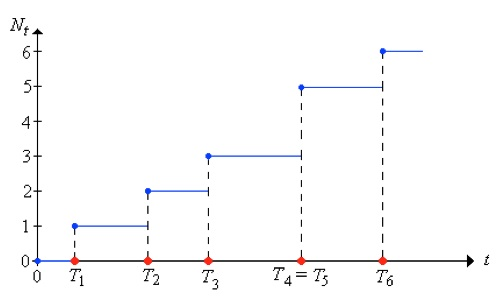
\includegraphics[width=5in]{renewal_process.jpg} 
   \caption{Renewal process (from  \cite{Che})}
   \label{rp}
\end{figure}


\begin{figure}[htbp] %  figure placement: here, top, bottom, or page
   \centering
   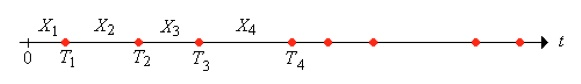
\includegraphics[width=5in]{renewal_process_2.jpg} 
   \caption{Renewal process (from \cite{Che})}
   \label{rp2}
\end{figure}

(This corresponds to installing a light bulb at $ t=0 $,  and subsequently immediately upon failure of the previous bulb.  Then the $ T_n $ are  the installation or renewal times.)

The associated \emph{renewal \underline{counting} process} $ (N_t)_{t\geq 0 }  $ is the number of renewals up to and including time $ t  $.  That is 
\begin{equation} \label{} 
N_t =   \card \{n : T_n \leq t \} = \sum_{n\geq 0} \mathbb{I}_{\{T_n \leq t\}}.
\end{equation} 
\hfill $\square$  \end{remark}

\begin{remark} 
The \emph{renewal function} and \emph{renewal measure} (both denoted $ U $) are  defined by 
\[
U(t) =  U[0,t] =\mathbb{E}\, N(t).
\]
This is the expected number of renewals up to time $ t $, and $ U(A) $ is the expected number of renewals in $ A $. Moreover,
\[
U[0,t] = \sum_{n\geq 0} \expected \mathbb{I}_{\{T_n \leq t \}} = \sum_{n\geq 0} P\{ T_n \leq t\} = \mu^{*n}[0,t] .
\] 
That is 
\begin{equation} \label{} 
U = \sum_{n\geq 0}  \mu^{*n}, \quad \text{where } \mu^{*0} = \delta _ 0 .
\end{equation} 
 Note $ T_0 = 0 $.   This also follows from Proposition~\ref{solre}. 

For $ t\geq 0 $,
\begin{align*}
U(t) &= \mathbb{E}_y\, \mathbb{E} \, (N(t) \mid X_1 = y ) \\
&= \mathbb{E} _y\, \big( 1 + U(t-y)\big) \quad \text{(since the process starts again at $ X_1 $)}\\
&= 1 + \int U(t-y)\, d\mu(y).
\end{align*}  
That is,  $ U $ satisfies the renewal equation \eqref{re} with $ g = \mathcal{X} _{[0,\infty)} $.

It follows from the renewal theorem   that in the non-arithmentic case, \emph{$ U $ is approximately a multiple of Lebesgue measure $ L^1 $}.  
More precisely,
 \begin{proposition}
 If $ \mu $ is non-arithmetic, then
 \[
 U[t,t+h] \to \lambda ^{-1} h \text{ as } t \to \infty ,
 \] 
 for every $ h > 0 $.  Moreover, if $ \mu $ is $ \tau $-arithmetic then the same is true provided $ h $ is a multiple of $ \tau $.
\end{proposition} 

\begin{proof} Let  $ g = \mathcal{X}_[0,h] $ in the Renewal Theorem~\ref{renthm}.
\end{proof} 
\end{remark} 

The renewal equation, under quite general conditions, has a unique solution given by an infinite series expansion.

More precisely, we make the following assumptions
*** these are only needed for the renewal theorem.  The following proposition is true under weaker hypotheses, sufficient to include 
the case with $ U(t) $ and $ g(t) $ as above ***
\begin{enumerate}
\item $ \lambda := \mathbb{E} \, (X) = \int _0^\infty  t \, d\mu(t) < \infty $, where $ \dist X = \mu $;


\item  $ \mu $ is not concentrated at $ 0 $;
\item $ |g(t) | \leq c e^{- \alpha |t| } $ for some $ \alpha > 0 $, and $ g $ has a discrete set of discontinuities (more generally, $ g $ is ``directly Riemann integrable'').
\end{enumerate}
Note that   condition (3) on $ g $ is \emph{not} satisfied in  in Example~\ref{lbe}.

Let $ \mathcal{F} $ be the set of Borel measurable $ f : \mathbb{R} \to \mathbb{R} $ such that $ f(t) \to 0 $ as $ t \to -\infty $ and $ f $ is bounded on each $ (-\infty, a ] $.

  \begin{proposition}[Solution of the renewal equation]\label{solre}
  Under the previous hypotheses *** and more generally as noted before ***  there is a unique solution of the renewal equation given by
  \begin{equation} \label{sre}
  \begin{aligned}
  f &= \sum_{n\geq 0} g * \mu^{*n} = g*U,\\
  \text{i.e.\ } f(t) &= \sum_{n\geq 0} \mathbb{E} \, g \big ( t - ( X_1 + \dots + X_n) \big) \\
  &= \sum_{n\geq 0} \int_0^\infty \cdots \int_0^\infty g(t - y_1 - \dots - y_n) \, d\mu(y_1)\ldots d\mu(y_n).
  \end{aligned} 
  \end{equation}
 Moreover, $ f $ is bounded, and if $ g $ is continuous then $ f $ is uniformly continuous.  
  \end{proposition} 
  
 \begin{proof} The formal idea is that if $ f(t) =  \sum_{n\geq 0} \big(g * \mu^{*n}\big) (t) $ then
  \begin{align*}
  f(t) &= g(t) + \sum_{n\geq 0} \big( ( g * \mu^{*n})*\mu \big) (t) \\
  &= g(t) + \int \sum_{n\geq 0} \big( g * \mu^{*n} \big) (t-y) \, d\mu(y) \\
  &= g(t) + \int f(t-y)\, d\mu(y).
  \end{align*} 
 The justification for the various steps and for the regularity results  follow from the hypotheses. 
  \end{proof} 
  
  For the  Renewal Theorem~\ref{renthm}             we will need to consider two cases for $ \mu $.
  
  \begin{definition} The measure $ \mu $ is \emph{$ \tau $-arithmetic} if 
  \[
   E:= \spt \mu \subset \{ a + \tau k : k \in \mathbb{N} \}
   \]
   for some $ a \in \mathbb{R} $ (take $ a\in [0,\tau) $ w.l.o.g.), and $ \tau $ is the greatest such positive number.
   
   Otherwise, $ \mu $ is \emph{non-arithmetic}.
 \end{definition}  
  
\begin{remark} \label{fdep} If $ \mu $ is $ \tau $-arithmetic and $ f $ satisfies the renewal equation, then it is clear from the first form of ~\eqref{re} that, for each \emph{fixed} $ t \in \mathbb{R} $, this gives a relationship involving only   
\[
f(t-k \tau),\ g(t), \ \mu\{k\tau\}, \quad \text{for } k \in \mathbb{N} _0.
\] 
Similarly, if $ f $ satisfies the renewal equation,  then it is clear from the second form of ~\eqref{sre} that, for each \emph{fixed} $ t \in \mathbb{R} $, this gives a relationship involving only   
\[
f(t),\ g(t-k \tau), \ \mu\{k\tau\}, \quad \text{for } k \in \mathbb{N} _0.   
\] 
  \end{remark} 
  
\begin{remark}\label{infpf}
  The renewal theorem below refers to the limit  behaviour of the solution $ f(t) $  to the renewal equation as $ t \to \infty $.
  Recall $ f(t) = \sum_{k\geq 0} \expected g\big(t-(X_1+\dots +X_n)\big) $.  
  
  Since $ f = g* U $ and $ U $ is asymptotically   $ L^1 $ normalised by the mean of $ \mu $, (at least in the non-arithmetic case) we expect that asymptotically $ f $ is the integral of $ g $ normalised by the mean of $ \mu $.  More carefully, we argue as follows.

\emph{Non-arithmetic case.} In order to find an approximation to $ f (t) $ for large $ t $, approximate $ g $ by a sum of functions of the form $ \alpha \mathcal{X} _{[a,b] } $.  First suppose $ g $ is itself a summand of this form, $ t >> b $ and $ b-a << \lambda $.  
The probability that $ t-(X_1+\dots +X_n) \in [a,b] $ for some $ n $ is approximately $ [b-a]/ \lambda $, and this is the same for the probability that $ t-(X_1+\dots +X_n) \in [a,b] $ for exactly one $ n $.  It follows that $ f(t) \approx  \alpha [b-a]/ \lambda $.  By summing, for general $ g $ it follows that $ f(t) \approx \lambda ^{-1} \int g(x)\, dx $. 

\emph{Arithmetic case.} In order to find an approximation to $ f (t) $ for large $ t $, it follows from  Remark~\ref{fdep}  that the relevant arguments for $ g $ are $ t-k\tau $ for $ k \in \mathbb{N} _0 $.  First suppose $ g ( t - k' \tau ) = \alpha $ for some $ k' $ and that otherwise $ g( t - k  \tau) = 0 $, and suppose $ t >> t-k'\tau$.  The probability that $ t - (X_1 + \dots + X_n ) = t - k'\tau $ for some (and hence exactly one) $ n $ is approximately $ 1/\lambda d$. It follows that $ f(t) \approx \lambda ^{-1} \alpha $.  By summing, for general $ g $, it follows that $ f(t) \approx \lambda ^{-1} \sum_{j=-\infty}^\infty g(t + j \tau )$.
    \hfill $\square$  \end{remark} 
    

\begin{theorem}[Renewal theorem] \label{renthm}  Suppose the hypotheses as for Proposition~\ref{solre} and that $ f \in \mathcal{F} $ is the solution of the renewal theorem.
If $ \mu $ is non-arithmetic then 
\begin{equation} \label{}
\lim_{x \to \infty } f(x) = \lambda ^{-1} \int g(t)\, dt  .
\end{equation}
If $ \mu $ is $ \tau$-arithmetic then for $ t_0 \in [0,\tau) $,
\begin{equation} \label{} 
\lim_{k\to \infty} f(t_0+ k\tau ) = \lambda ^{-1} \sum_{j=-\infty}^\infty g(t_0 + j \tau ).
\end{equation} 
\end{theorem}   

\begin{proof}
\textbf{Method 1.} This makes rigorous the informal argument in Remark~\ref{infpf} by using acoupling argument.

\bigskip 
\noindent \textbf{Method 2.} We outline the non arithmetic case.

\noindent \emph{Step (a).}  From \eqref{re} one gets
\[
\int_{-\infty}^x g(t)\, dt = \int f(t)\, \psi(x-t)\, dt = (f*\psi)(x) \quad \text{where }   \psi(t) = \begin{cases} 0 & t< 0 \\ \mu[t,\infty) &t \geq 0 \end{cases}.
\]
 
 \medskip \noindent \emph{Step (b).} Hence
 \[
 (f * \psi)(x) \to \int g(t)\, dt \quad \text{as } x \to \infty .
 \]
 (Think of $ (f*\psi) (x)$  as a weighted average of   values of $ f $ at points $ y < x $.)
 
 \medskip \noindent \emph{Step (c).} By Wiener's theorem, since we can show $ \widehat{\psi} (u) \neq 0 $, 
 \[
 (f * \phi)(x) \to \frac{\int \phi}{\int \psi} \int g(t)\, dt \quad \text{as } x \to \infty,
 \]
 for \emph{any} $ \phi \in L^1( \mathbb{R} ) $.
 
 We can check that $   \int \psi = \lambda $.

 \medskip \noindent \emph{Step (d).} Setting $ \phi $ to be an approximation to the Dirac $ \delta $-function and using the uniform continuity of $ f $, it follows that
 \[ 
 f(x) \to \lambda ^{-1} \int g(t)\, dt \quad \text{ as } x \to \infty .
 \]
 
  \medskip \noindent \emph{Step (e).} If $ g $ has  a discrete set of discontinuities, then we   approximate $ g $ by continuous functions.
 
\medskip (Arithmetic case?)
\end{proof} 

We use the following, which is just a restatement of the previous theorem   for $ \mu $ with finite discrete support.

\begin{corollary}
Suppose $ m \geq 2 $, $ t_1,\dots, t_m >0 $ are ``times'', and $ p_1,\dots , p_m $ are probabilities, so that $ \sum_i p_i = 1 $. Let $ g $ be as before Proposition~\ref{solre} and let $ f $ satisfy the renewal equation
\begin{equation} \label{} 
f(t) = g(t) + \sum_i p_i f(t - t)i).
\end{equation} 
Let $ \lambda = \sum_i p_i t_i $.

If  $ \{t_1,\dots, t_m \} $ is non-arithmetic then 
\[
\lim_{t\to \infty} f(t) = \lambda ^{-1} \int g(t)\, dt.
\]
If $ \{t_1,\dots, t_m \} $ is $ \tau $-arithmetic then 
\[
\lim_{ k \to \infty}  f(t_0 + k\tau ) =  \lambda ^{-1} \sum_{k=-\infty}^\infty g(t_0 + k\tau ),
\]
for all $ t_0 \in [0,\tau) $.
\end{corollary} 


%%%%%%%%%%%%%%%%%%%%%%%%%%%%%%%%
%%%%%%%%%%%%%%%%%%%%%%%%%%%%%%%%
%%%%%%%%%%%%%%%%%%%%%%%%%%%%%%%%
%%%%%%%%%%%%%%%%%%%%%%%%%%%%%%%%
\section{CJM Processes}

\subsection{Notation and Non-probabilistic aspects}

Consider a population of individuals with an \emph{initial ancestor} denoted by $ \phi $.  This individual will have a finite number of children, each of these  will have a finite number of children, etc.  Each individual apart from the initial ancestor  has exactly one parent and there is no notion of breeding in this model.

(Later we will impose  a notion  of absolute time,  and of birth and death times.) 

\medskip The set of all individuals (alive or dead) is naturally represented by a \emph{tree} $ T \subset \bigcup_{k\geq 0 } \mathbb{N}  ^k $, where $ \mathbb{N} ^0 = \{ \emptyset \} $ and $ \mathbb{N} ^k $ is the set of finite sequences $ \boldsymbol{i} = i_1\dots i_k $ of positive integers.
We  use the standard notations $ | \boldsymbol{i} |$ for the length of $ \boldsymbol{i} $, $ \boldsymbol{i} |_k $ for truncation and $ \boldsymbol{i} \boldsymbol{j} $ for concatentation.

Motivated by the above we require:
\begin{enumerate}
\item $ \emptyset \in T $;
\item $ \boldsymbol{i} \in T $ implies (the unique $ k $th generation ancestor)  $ \boldsymbol{i} |_k \in T $ for $ k < | \boldsymbol{i}| $;
\item $ \boldsymbol{i} 1,\dots ,  \boldsymbol{i} N^{ \boldsymbol{i} }  \in T $ and $\boldsymbol{i} (N^{ \boldsymbol{i} }+1), \boldsymbol{i} (N^{ \boldsymbol{i} }+2), \dots \notin T $, where $  N^{ \boldsymbol{i} } $ is the \emph{number of children of $ \boldsymbol{i} $}.
\end{enumerate} 

\medskip Associated with each $ \boldsymbol{i} \in T $ is a \emph{life-story} $ U^{ \boldsymbol{i} } = (L^{ \boldsymbol{i} }, \xi^{ \boldsymbol{i} } ) $ where 
\begin{enumerate}
\item $ L^{ \boldsymbol{i} } \in [0,\infty) $  is the \emph{lifetime} of $ \boldsymbol{i} $;
\item $ \xi ^ { \boldsymbol{i} } : [0,\infty) \to \mathbb{N} _ 0 $% 
\footnote{$ \mathbb{N} _ 0 $ is the set of natural numbers together with $ 0 $.} 
is a bounded non-decreasing right-continuous function, and $ \xi ^{ \boldsymbol{i} } ( t) $ is the number of births  from  $ \boldsymbol{i} $ up to and including time $ t $. 
We \emph{assume} $ \xi (0) = 0 $.
\end{enumerate} 

The jumps in $ \xi ^ {\boldsymbol{i} } $ determine age $ t^{ \boldsymbol{i} }(j) $ of $ \boldsymbol{i} $ at the birth of   the $ j $th child of $ \boldsymbol{i} $. The number of births at age  $ t $ is the  size of the jump at $ t $. The  total number of births  for $ \boldsymbol{i} $ is denoted $ N^{ \boldsymbol{i} }$.  The   ages at time of berth  satisfy 
\begin{equation} \label{tseq}  
0 < t^{ \boldsymbol{i} }(1) \leq t^{ \boldsymbol{i} }(2) \leq \dots \leq  t^{ \boldsymbol{i} }(N^{ \boldsymbol{i} })\leq L^{ \boldsymbol{i} } .
\end{equation} 

More precisely,    \emph{define}
\begin{equation} \label{} 
N^{ \boldsymbol{i} } := \xi [0,\infty), \quad t^{ \boldsymbol{i} } (j) := \inf \{ t : \xi^ {\boldsymbol{i}  } (t) \geq j \}.
\end{equation} 
We also  w.l.o.g.\ make the assumption
\begin{equation} \label{} 
 t^{ \boldsymbol{i} }(N^{ \boldsymbol{i} }) \leq L^{ \boldsymbol{i} } .
\end{equation} 

Then \eqref{tseq} follows, as does
\begin{equation} \label{} 
\xi ^{ \boldsymbol{i} } (t) = \max \big\{ j : t^{ \boldsymbol{i} } (j) \leq t \big\}.
\end{equation} 
See Figure~\ref{rp}, where    a different notation is used.  

 
 In the usual way, $   \xi ^ { \boldsymbol{i}  } $  is the distribution function for a measure, also denoted by $    \xi ^ { \boldsymbol{i}  } $. 
Thus
\[
\xi ^ { \boldsymbol{i} } (s,t] = \xi ^ { \boldsymbol{i} } (t) - \xi ^ { \boldsymbol{i} } (s) ,  \quad \xi ^ { \boldsymbol{i} } (t) =  \xi ^ { \boldsymbol{i} } (0,t] .
\]
The measure $ \xi^ { \boldsymbol{i} } $ is a sum of Dirac measures, one for each birth and counted with multiplicities.  More precisely,
\begin{equation} \label{} 
\xi ^ { \boldsymbol{i} } = \sum_{j=1}^{ N^ { \boldsymbol{i} }} \delta _{ t^{ \boldsymbol{i} } (j) }.
\end{equation} 

\medskip The \emph{time  at the birth} of an individual is defined recursively by
\begin{equation} \label{} 
\sigma_{ \emptyset} = 0, \quad \sigma_{ \boldsymbol{i} j }  = \sigma _{ \boldsymbol{i} } + t^{ \boldsymbol{i} } (j).
\end{equation} 
Thus if we attach the time $ t^{ \boldsymbol{i} }(j) $ to the edge from $ \boldsymbol{j} $ to $ \boldsymbol{j} k $ then the time at birth of $ \boldsymbol{i} $ is the sum of the times along all edges in $ i_1\dots i _{ | \boldsymbol{i} |} $.  That is
\begin{equation} \label{tb} 
\sigma_{ \boldsymbol{i} } = t^{ \emptyset} (i_1) + t^{i_1}(i_2) + \dots + t^{i_1\dots i_{n-1} }(i_n) 
= \sum_{k=1}^n t^{ i_1\dots i_{k-1}}(i_k) 
\quad \text{if } | \boldsymbol{i} | = n \geq 1 .
\end{equation} 


\begin{example}
We use standard notation.

Consider a fractal set indexed by a tree $ T $ in the usual manner.  That is, the  $ n $-cell $\Delta_{\boldsymbol{i}}$ is replaced by  a scaled copy of $ F^{ \boldsymbol{i} }(G_0) =  \bigcup_{j=1}^M f^{ \boldsymbol{i} }_j(G_0) $, where $ F^{ \boldsymbol{i} } = \{f^{ \boldsymbol{i} }_1,\dots, f^{ \boldsymbol{i} }_M\} $ is an IFS of similarities in $ \mathbb{R}^k $ with contraction ratios $ \ell^{ \boldsymbol{i} }_1\geq \dots \geq  \ell^{ \boldsymbol{i} }_M $. 

In this case the ages of $ \boldsymbol{i} $ at   times of giving birth and at death  are  defined by
\[
 t^{ \boldsymbol{i} } (j) = \log 1/\ell^{ \boldsymbol{i} } _j, \quad L^{ \boldsymbol{i} } = \log 1/ \ell^{ \boldsymbol{i} } _M .
\]
 In particular,  from \eqref{tb} by setting
\[
t^{ \boldsymbol{i} }(j) = \log \left(\ell^{ \boldsymbol{i} }_j \right)^{-1}, \quad \ell^{ \boldsymbol{i} }_j  = \exp \left( - t^{ \boldsymbol{i} }(j)  \right),
\]
it follows that 
  the time at birth of the cell $ \boldsymbol{i} $ is 
\begin{equation} \label{}
\sigma_{\boldsymbol{i}  } = \log \ell_{ \boldsymbol{i} }^{-1}, \quad \text{i.e.\ }  \ell_{ \boldsymbol{i} } = \exp \left( - \sigma_{\boldsymbol{i}  } \right),
\end{equation}
where as usual $ 
\ell_{ \boldsymbol{i} } := \prod_{k=1}^n \ell^{ i_1\dots i_{k-1}}_{i_k} $ 
if $ | \boldsymbol{i} | = n $. 

Note for future reference that  if $ F:= \{ f_1,\dots f_m \} $ and $ t_j := \log \ell_j^{-1} $ then  
\begin{equation} \label{}
\sum_j \ell^ \alpha _j = 1 \Longleftrightarrow  \sum_j e^{- \alpha t_j  } \ \left(\text{i.e.} \int_0^\infty e^{- \alpha t} \xi (dt) \right) 
= 1 ,
\end{equation}
and more generally
\begin{equation} \label{}
\sum_{\boldsymbol{i} \in \Lambda } \ell_{ \boldsymbol{i} }^ \alpha  = 1 \Longleftrightarrow 
                \sum_{\boldsymbol{i} \in \Lambda } e^{ - \alpha \sigma _{ \boldsymbol{i} }} = 1.
\end{equation} 



\end{example} 

%%%%%%%%%%%%%%%%%%%%%%%%%%%%%%%%
%%%%%%%%%%%%%%%%%%%%%%%%%%%%%%%%
%%%%%%%%%%%%%%%%%%%%%%%%%%%%%%%%
%%%%%%%%%%%%%%%%%%%%%%%%%%%%%%%%


\begin{thebibliography}{9} 

\bib{Ash}{book}{
   author={Ash, Robert B.},
   title={Probability and measure theory},
   edition={2},
   note={With contributions by Catherine Dol\'eans-Dade},
   publisher={Harcourt/Academic Press, Burlington, MA},
   date={2000},
   pages={xii+516},
%   isbn={0-12-065202-1},
%   review={\MR{1810041 (2001j:28001)}},
}

 \bib{Che}{misc}{
  author={Chen, Kani},
  note = {online notes},
  date={2009},
  title={Advanced probability Math 541},
  }
  
  \bib{Fal}{book}{
   author={Falconer, Kenneth},
   title={Techniques in fractal geometry},
   publisher={John Wiley \& Sons Ltd.},
%   place={Chichester},
   date={1997},
   pages={xviii+256},
%   isbn={0-471-95724-0},
%   review={\MR{1449135 (99f:28013)}},
} 

  \bib{Fel}{book}{
   author={Feller, William},
   title={An Introduction to probability Theory and its Applications},
   edition={2},
   publisher={Wiley},
   date={1971},
   pages={xxiv+669},
%   isbn={0-12-065202-1},
%   review={\MR{1810041 (2001j:28001)}},
}

  
\bib{Lam}
{book}{
   author={Lamperti, John},
   title={Probability. A survey of the mathematical theory},
   publisher={W. A. Benjamin, Inc., New York-Amsterdam},
   date={1966},
   pages={x+150},
%   review={\MR{0206996 (34 \#6812)}},
}	

\end{thebibliography}

\end{document} 

